\documentclass{article}\usepackage[]{graphicx}\usepackage[]{xcolor}
% maxwidth is the original width if it is less than linewidth
% otherwise use linewidth (to make sure the graphics do not exceed the margin)
\makeatletter
\def\maxwidth{ %
  \ifdim\Gin@nat@width>\linewidth
    \linewidth
  \else
    \Gin@nat@width
  \fi
}
\makeatother

\definecolor{fgcolor}{rgb}{0.345, 0.345, 0.345}
\newcommand{\hlnum}[1]{\textcolor[rgb]{0.686,0.059,0.569}{#1}}%
\newcommand{\hlsng}[1]{\textcolor[rgb]{0.192,0.494,0.8}{#1}}%
\newcommand{\hlcom}[1]{\textcolor[rgb]{0.678,0.584,0.686}{\textit{#1}}}%
\newcommand{\hlopt}[1]{\textcolor[rgb]{0,0,0}{#1}}%
\newcommand{\hldef}[1]{\textcolor[rgb]{0.345,0.345,0.345}{#1}}%
\newcommand{\hlkwa}[1]{\textcolor[rgb]{0.161,0.373,0.58}{\textbf{#1}}}%
\newcommand{\hlkwb}[1]{\textcolor[rgb]{0.69,0.353,0.396}{#1}}%
\newcommand{\hlkwc}[1]{\textcolor[rgb]{0.333,0.667,0.333}{#1}}%
\newcommand{\hlkwd}[1]{\textcolor[rgb]{0.737,0.353,0.396}{\textbf{#1}}}%
\let\hlipl\hlkwb

\usepackage{framed}
\makeatletter
\newenvironment{kframe}{%
 \def\at@end@of@kframe{}%
 \ifinner\ifhmode%
  \def\at@end@of@kframe{\end{minipage}}%
  \begin{minipage}{\columnwidth}%
 \fi\fi%
 \def\FrameCommand##1{\hskip\@totalleftmargin \hskip-\fboxsep
 \colorbox{shadecolor}{##1}\hskip-\fboxsep
     % There is no \\@totalrightmargin, so:
     \hskip-\linewidth \hskip-\@totalleftmargin \hskip\columnwidth}%
 \MakeFramed {\advance\hsize-\width
   \@totalleftmargin\z@ \linewidth\hsize
   \@setminipage}}%
 {\par\unskip\endMakeFramed%
 \at@end@of@kframe}
\makeatother

\definecolor{shadecolor}{rgb}{.97, .97, .97}
\definecolor{messagecolor}{rgb}{0, 0, 0}
\definecolor{warningcolor}{rgb}{1, 0, 1}
\definecolor{errorcolor}{rgb}{1, 0, 0}
\newenvironment{knitrout}{}{} % an empty environment to be redefined in TeX

\usepackage{alltt}
\usepackage{amsmath} %This allows me to use the align functionality.
                     %If you find yourself trying to replicate
                     %something you found online, ensure you're
                     %loading the necessary packages!
\usepackage{amsfonts}%Math font
\usepackage{graphicx}%For including graphics
\usepackage{hyperref}%For Hyperlinks
\usepackage[shortlabels]{enumitem}% For enumerated lists with labels specified
                                  % We had to run tlmgr_install("enumitem") in R
\hypersetup{colorlinks = true,citecolor=black} %set citations to have black (not green) color
\usepackage{natbib}        %For the bibliography
\setlength{\bibsep}{0pt plus 0.3ex}
\bibliographystyle{apalike}%For the bibliography
\usepackage[margin=0.50in]{geometry}
\usepackage{float}
\usepackage{multicol}

%fix for figures
\usepackage{caption}
\newenvironment{Figure}
  {\par\medskip\noindent\minipage{\linewidth}}
  {\endminipage\par\medskip}
\IfFileExists{upquote.sty}{\usepackage{upquote}}{}
\begin{document}

\vspace{-1in}
\title{Lab 7/8 -- MATH 240 -- Computational Statistics}

\author{
  Sankalp Ojha \\
  Colgate University  \\
  Mathematics  \\
  {\tt sojha@colgate.edu}
}

\date{04/03/2025}

\maketitle

\begin{multicols}{2}
\begin{abstract}
In this lab, we explored the Beta distribution. We explored the parameters and properties of the Beta distribution. We also explored the use of two point estimators, Method of Moments (MOM) and Maximum Likelihood Estimator (MLE), and how to check their accuracy. The point estimation methods were tested with real world data. We concluded that the MLE is better at finding the appropriate $\alpha$ and $\beta$ values compared to MOM.
\end{abstract}

\noindent \textbf{Keywords:} Beta distribution, MOM, MLE, $\alpha$, and $\beta$

\section{Introduction To Beta Distributions}
The Beta distribution is a continuous distribution. The Beta distribution models the behavior of a random variable $X$ within the support of 0 to 1. The Beta distribution is widely known for its flexibility, which makes it useful to model various datasets, probabilities, etc. Depending on the values of the parameters $\alpha$ and $\beta$, which will be discussed furthered in section 2, the Beta distribution can take on left-skewed, right-skewed, U-shaped, or symmetric shapes, as seen in \autoref{plot0}. Section 2 provides a greater description for the parameters for the Beta distribution. Section 3 discusses the properties and statistics of the Beta distribution. Sections 4 and 5 discusses point estimators and three metrics which we can use to check how accurate the estimators are, followed by a real world example of the use case for the estimators and checking metrics.

\section{Density Functions and Parameters}
A continuous distribution is one which has probability density function (PDF) and a cumulative density function (CDF) to represent its probability. The Beta distribution has two parameters, $\alpha$ and $\beta$, which dictate on the distribution looks. Both $\alpha$ and $\beta$ are positive numbers and correspond to \texttt{shape1} and \texttt{shape2}, respectively, when write code for the Beta distribution in \texttt{R}. The Beta distribution PDF is given as:

\[f_X(x|\alpha, \beta) = \frac{\Gamma(\alpha + \beta)}{\Gamma\alpha\Gamma\beta} x^{\alpha-1}(1-x)^{\beta-1}I(x \in [0,1]).\]

\indent In the beta distribution, $I(x \in [0,1]) = 1$ when $x \in [0,1]$ and $0$ whenever $x$ does not hold a number in support on the Beta distribution. The support of a random variable $X$ in the Beta distribution is $[0,1]$.

\section{Properties and Key Statistics}
The Beta distribution is a very versatile and flexible function when it comes to the shapes it can take on based on the various values of the $\alpha$ and $\beta$ parameters. The various forms of the Beta distribution can be shown through statistics such as mean, variance, skewness, and excess kurtosis. Something to note about the \verb|kurt()| function in \texttt{R} is that it computes the excess kurtosis. So, if we are interested in finding kurtosis of a distribution, we can simply add three to the excess kurtosis found through the \verb|kurt()| function. The equations which can be used to calculate the statistics for a Beta distribution are written in terms of $\alpha$ and $\beta$, as seen below:

\begin{align*}
 E(X) = \frac{\alpha}{\alpha + \beta} \tag{The Mean}\\
var(X) = \frac{\alpha\beta}{(\alpha + \beta)^2(\alpha + \beta + 1)} \tag{The Variance} \\
skew(X) = \frac{2(\beta - \alpha)\sqrt{\alpha + \beta + 1}}{(\alpha + \beta + 2)\sqrt{\alpha\beta}} \tag{The Skewness}
\end{align*}
\[kurt(X) = \frac{6[(\alpha - \beta)^2(\alpha + \beta + 1) - \alpha\beta(\alpha + \beta + 2)]}{\alpha\beta(\alpha + \beta + 2)(\alpha + \beta + 3)}\]
\begin{flushright}
(The Excess Kurtosis)
\end{flushright}

\autoref{table2} tables all the summary statistics for the various Beta distributions seen in \autoref{plot0} and illustrates how the $\alpha$ and $\beta$ dictate the shape of the Beta distribution.

Another way to compute these statistics is through their centered and uncentered $k$th moments. We can compute various combinations of centered and uncentered $k$th moments of the Beta distribution to calculate a certain statistic, as seen below:

\begin{align*}
 \mu_X = E(X) \tag{The Mean}\\
 var(X) = \sigma^2_X = E[(X-\mu_X)]^2 \tag{The Variance}\\
 skew(X) = \frac{E[(X - \mu_X)^3]}{E[(X-\mu_X)^2]^{3/2}} \tag{The Skewness}\\
 kurt(X) = \frac{E[(X-\mu_X)^4]}{E[(X-\mu_X)^2]^2} - 3 \tag{The Excess Kurtsosis}
\end{align*}

To generalize these equations to calculate any centered or uncentered $k$th moment of the Beta distribution, we can use the equations

\[E(X^{k}) = \int_{\chi}^{} x^{k}f_x(x) \,dx \]
\begin{center}
and 
\end{center}
\[E((X-\mu_X)^{k}) = \int_{\chi}^{} (x-\mu_X)^{k}f_x(x) \,dx \]

where the first equation corresponds to a centered $k$th moment and the second equation corresponds to a uncentered $k$th moment.

For the purposes of this lab, a function \verb|beta.moment(alpha, beta, k, centered)| was made to calculate the various statistics of the Beta distribution for various values of $\alpha$ and $\beta$.

\subsection{Power of Larger Sample Sizes}
By generating a large random sample from a fixed Beta distribution with parameters $\alpha = 2$ and $\beta = 5$, we were able to prove that larger random sample sizes converge closer to the exact distribution. Using the \texttt{cumstats} package \citep{cumstats}, I made \autoref{plot1}, which illustrates how the Weak Law Of Large Numbers works. The Weak Law Of Large Numbers suggests that as the sample size increases so will the precision increase towards the total population distribution.

\section{Estimators And Precision}
When dealing with data in real world applications, we don't necessarily know what the values of the parameters $\alpha$ and $\beta$ will be for the given data set. This is where we use point estimators to calculate the precise values of $\alpha$ and $\beta$ which will best fit the data set. The two methods to estimate include: Method of Moments (MOM) and Maximum Likelihood Estimation (MLE). The MOM approach equates the first sample $k$th moments to the first population $k$th moments. The goal is to find which values of $\alpha$ and $\beta$ will match the data set moments best with the population moments. The MLE approach utilizes a likelihood function which aims to find the values of $\alpha$ and $\beta$ which will maximize the likelihood of matching the shape given data set. In \texttt{R}, to compute the values of $\alpha$ and $\beta$ using MOM, we first make a function which returns the first population $k$th moments minus the first sample $k$th moments. Then we used the \texttt{nleqslv} package \citep{nleqslv} and the function \verb|nleqslv()| to solve for the values of $\alpha$ and $\beta$ which make first population $k$th moments minus the first sample $k$th moments equal to zero. The MLE is implemented through a function which is passed into \verb|optim()|. The \verb|optim()| function maximizes the negative log-likelihood function. As both of these methods are estimates, we would like to know how precise the estimates are, which we can do through calculating Bias, Precision, and Mean Squared Error (MSE). Bias calculates the average difference from the true value, precision calculates the consistency of the estimates, and MSE combines both prior metrics to calculate the error. The equations to calculate each measure are:

\[\text{Bias} = \mathbb{E}(\hat{\theta}) - \theta\]
\[\text{Precision} = \frac{1}{\text{Var}(\hat{\theta})}\]
\[\text{MSE} = \text{Var}(\hat{\theta}) + \left( \mathbb{E}(\hat{\theta}) - \theta \right)^2\]

\noindent where $\boldsymbol{\hat{\theta}}$ is a given vector of estimates and $\boldsymbol{\theta}$ is the true value.

\section{Example: World Death Rates}
The study, \cite{faith}, suggests the worldwide death rates can be modeled by a Beta distribution with the specific parameters, $\alpha = 8$ and $\beta = 950$. Using the MOM and MLE estimator methods, we calculated the $\alpha$ and $\beta$ which would best fit the dataset for 1000 random samples of of size $n = 266$ for world death rates. To check which estimator is more accurate, we can use Bias, Precision, and MSE. Below is a table information about the accuracy of each estimator:

\begin{Figure}
\centering
\begin{tabular}{rllrrr}
  \hline
 parameters & method & bias & precision & mse \\ 
  \hline
    Alpha & MOM & 0.08 & 1.83 & 0.55 \\ 
    Alpha & MLE & 0.07 & 2.13 & 0.48 \\ 
    Beta & MOM & 10.29 & 0.00 & 8288.46 \\ 
    Beta & MLE & 9.11 & 0.00 & 7132.70 \\ 
   \hline
\end{tabular}
\captionof{table}{MOM and MLE bias, precision, and MSE for $\alpha$ and $\beta$.}
\label{table1}
\end{Figure}

As can be seen in the table, the MLE estimator is the more precise estimator. In the Bias, Precision, and MSE categories, MLE had lower numbers than MOM. This indicates that MLE is less bias, more precise, and overall a more accurate point estimator tool. It should be noted that the precision calculations for MOM and MLE $\beta$ were extremely small and are represented as zero as a result. While both methods are not fully accurate, MLE proves to be the superior method.

%%%%%%%%%%%%%%%%%%%%%%%%%%%%%%%%%%%%%%%%%%%%%%%%%%%%%%%%%%%%%%%%%%%%%%%%%%%%%%%%
% Bibliography
%%%%%%%%%%%%%%%%%%%%%%%%%%%%%%%%%%%%%%%%%%%%%%%%%%%%%%%%%%%%%%%%%%%%%%%%%%%%%%%%
\vspace{2em}
\begin{tiny}
\bibliography{bib7}
\end{tiny}
\end{multicols}

%%%%%%%%%%%%%%%%%%%%%%%%%%%%%%%%%%%%%%%%%%%%%%%%%%%%%%%%%%%%%%%%%%%%%%%%%%%%%%%%
% Appendix
%%%%%%%%%%%%%%%%%%%%%%%%%%%%%%%%%%%%%%%%%%%%%%%%%%%%%%%%%%%%%%%%%%%%%%%%%%%%%%%%
\newpage
\onecolumn
\section{Appendix}

\begin{figure}[ht]
  \begin{center}
  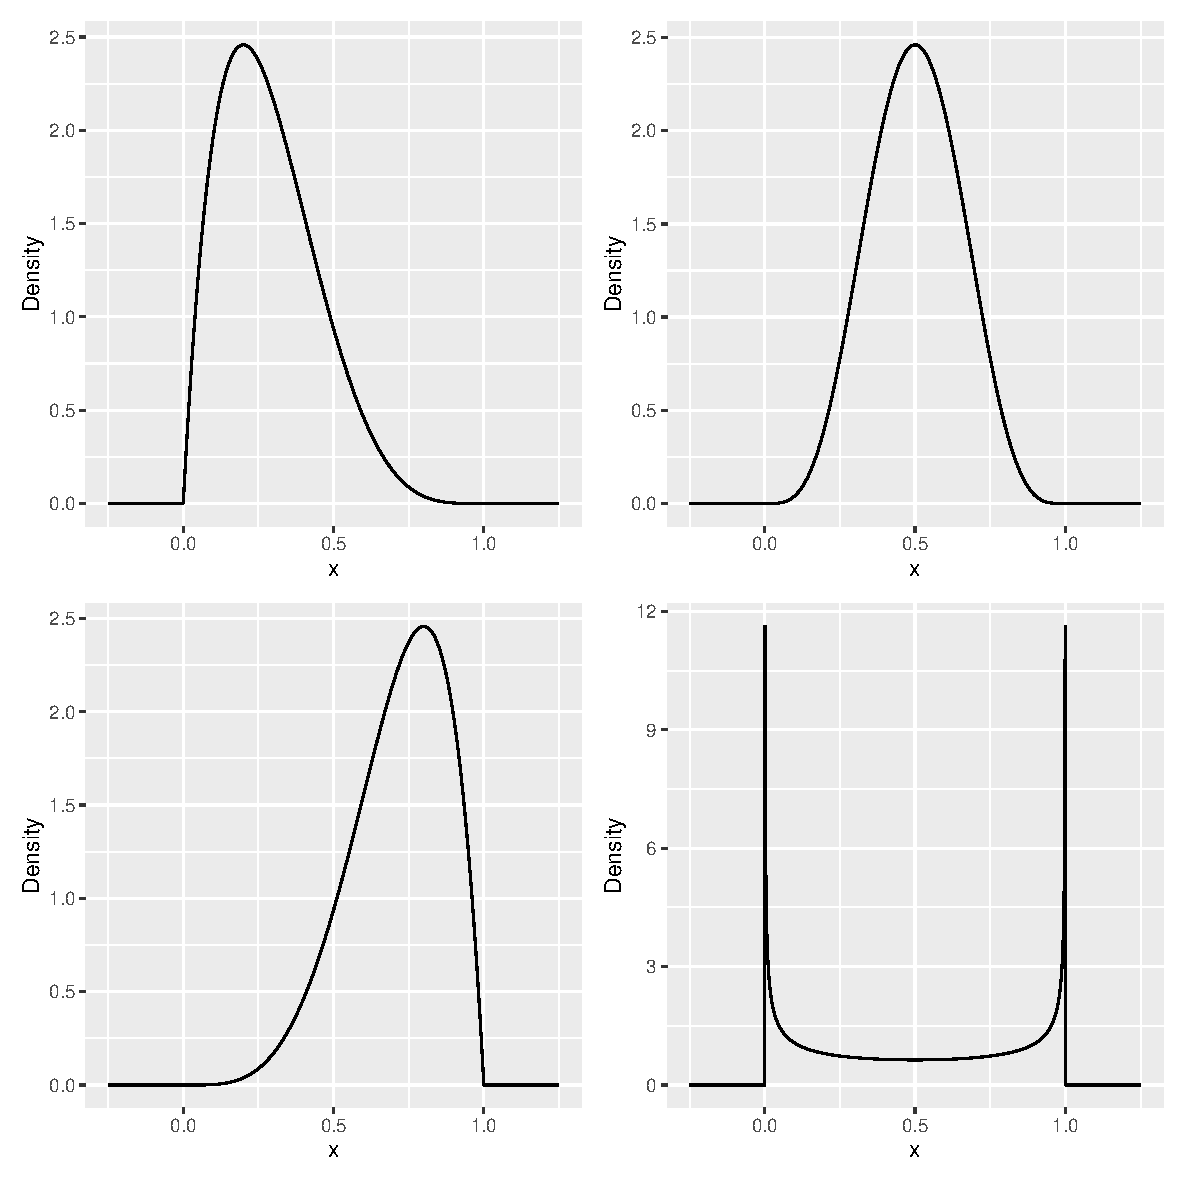
\includegraphics[width=\textwidth]{Rplot03.pdf}
  \caption{Plotting various beta PDFs with varying $\alpha$ and $\beta$ values.}
  \label{plot0}
  \end{center}
\end{figure}

\begin{table}[ht]
\centering
\caption{Population Summary Of 4 Beta Distribution Parameters with varying $\alpha$ and $\beta$ values.}
\label{table2}
\begin{tabular}{rrrrrrr}
  \hline
 & Alpha & Beta & Mean & Variance & Skewness & Excess Kurtosis \\ 
  \hline
1 & 2.00 & 5.00 & 0.29 & 0.03 & 0.60 & -0.12 \\ 
  2 & 5.00 & 5.00 & 0.50 & 0.02 & 0.00 & -0.46 \\ 
  3 & 5.00 & 2.00 & 0.71 & 0.03 & -0.60 & -0.12 \\ 
  4 & 0.50 & 0.50 & 0.50 & 0.12 & 0.00 & -1.50 \\ 
   \hline
\end{tabular}
\end{table}

\begin{figure}[ht]
  \begin{center}
  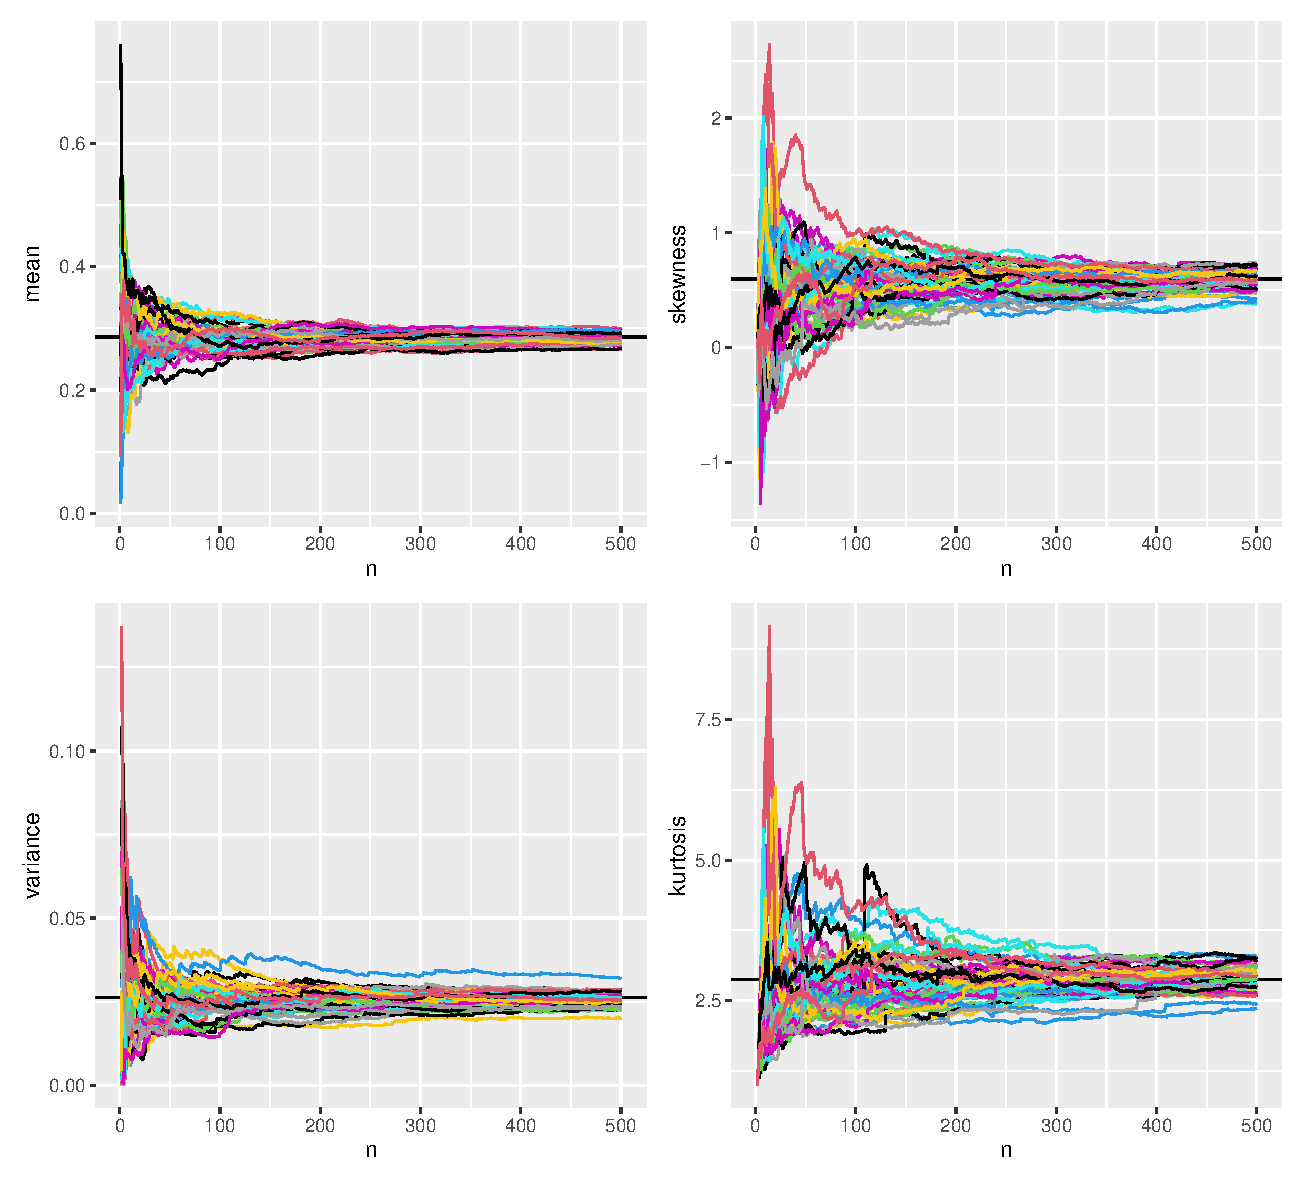
\includegraphics[width=\textwidth]{Rplot.pdf}
  \caption{$\alpha$=2 and $\beta$=5 convergence simulation to show the weak law of large numbers.}
  \label{plot1}
  \end{center}
\end{figure}

\begin{figure}[ht]
  \begin{center}
  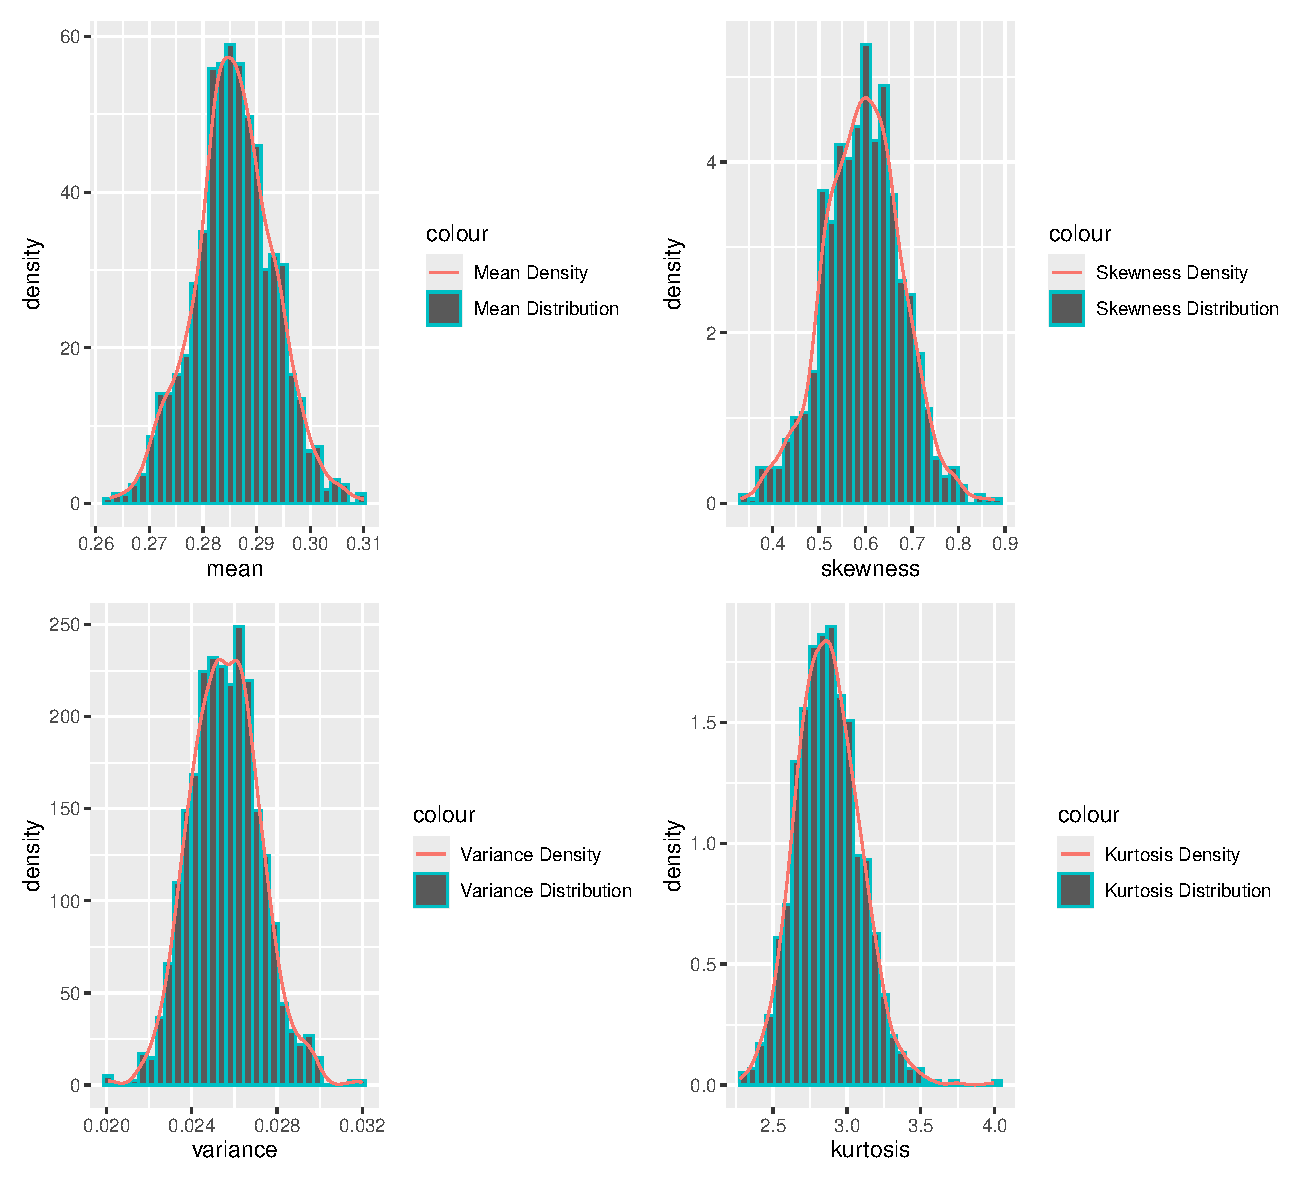
\includegraphics[width=\textwidth]{Rplot01.pdf}
  \caption{Beta($\alpha$=2 and $\beta$=5) sampling distributions to illustrate various summary statistics.}
  \label{plot2}
  \end{center}
\end{figure}

\begin{figure}[ht]
  \begin{center}
  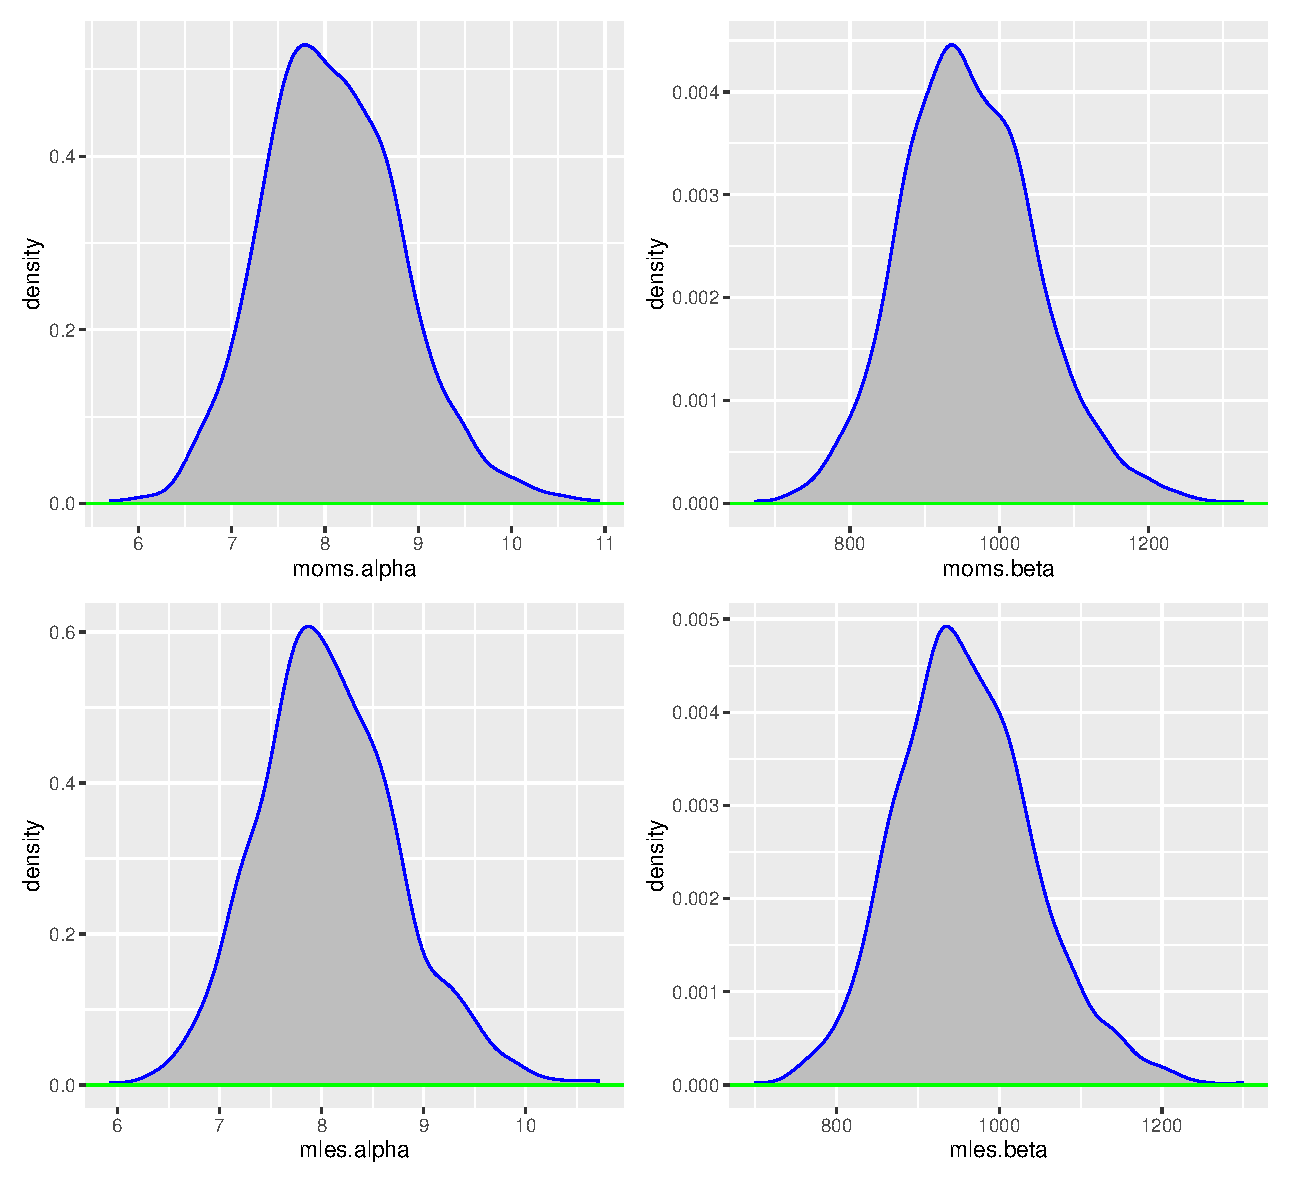
\includegraphics[width=\textwidth]{Rplot02.pdf}
  \caption{Resampled beta($\alpha$=8 and $\beta$=950) sampling distributions to illustrate the shape parameters behavior.}
  \label{plot3}
  \end{center}
\end{figure}

\end{document}
